% ŠABLONA PRO PSANÍ ZÁVĚREČNÉ STUDIJNÍ PRÁCE
%%%%%%%%%%%%%%%%%%%%%%%%%%%%%%%%%%%%%%%%%%%%
% Autor: Jakub Dokulil (kubadokulil99@gmail.com)
% Tato šablona byla vytvořena tak, aby pomocí ní mohli v systému LaTeX soutěžící sázet své práce a zároveň odpovídala požadavkům na formátování vyplývajícím z wordové šablony umístěné na webu soc.cz.
%
\documentclass[12pt, a4paper,
%oneside,      %% -- odkomentujte, pokud chcete svou práci mít pouze jednostrannou, mezera pro hřbet pak automaticky bude pouze na levé straně
twoside,        %% -- pro oboustranné práce, mezera pro hřbet následně střídá strany.
openright
]{report}

%% Nutné balíčky a nastavení
%%%%%%%%%%%%%%%%%%%%%%%%%%%%





%% Proměnné
\newcommand\obor{INFORMAČNÍ TECHNOLOGIE} %% -- napiš číslo a název tvého oboru
\newcommand\kodOboru{18-20-M/01} %% -- napiš číslo a název tvého oboru
\newcommand\zamereni{se zaměřením na počítačové sítě a programování} %% -- napiš číslo a název tvého oboru
\newcommand\skola{Střední škola průmyslová a umělecká, Opava} %% vyplň název školy
\newcommand\trida{IT4} %% vyplň jméno svého konzultanta
\newcommand\jmenoAutora{Sofja Klopcová}  %% vyplň své jméno
\newcommand\skolniRok{2023/24} %% vyplň rok
\newcommand\datumOdevzdani{1. 1. 2024} %% vyplň rok
\newcommand\nazevPrace{Robotické rameno ovládáné pomocí gest} %% vyplň název své práce
\let\oldchapter\chapter
\renewcommand{\chapter}{
	\clearpage
	\pagestyle{fancy}
	\fancyhf{}
	\renewcommand{\headrulewidth}{0pt}
	\fancyfoot[c]{\thepage}
	\
	\oldchapter
}



\title{\nazevPrace} %% -- Název tvé práce
\author{\jmenoAutora} %% -- tvé jméno
\date{\datumOdevzdani} %% -- rok, kdy píšeš SOČku

\usepackage[top=2cm, bottom=2.5cm, left=3.5cm, right=2cm]{geometry} %% nastaví okraje, left -- vnitřní okraj, right -- vnější okraj

\usepackage[czech]{babel} %% balík babel pro sazbu v češtině
\usepackage[utf8]{inputenc} %% balíky pro kódování textu
\usepackage[T1]{fontenc}
%\usepackage{cmap} %% balíček zajišťující, že vytvořené PDF bude prohledávatelné a kopírovatelné

\usepackage{graphicx} %% balík pro vkládání obrázků

\usepackage{subcaption} %% balíček pro vkládání podobrázků

\usepackage{hyperref} %% balíček, který v PDF vytváří odkazy

\linespread{1.25} %% řádkování
\setlength{\parskip}{0.5em} %% odsazení mezi odstavci


\usepackage[pagestyles]{titlesec} %% balíček pro úpravu stylu kapitol a sekcí
\titleformat{\chapter}[block]{\scshape\bfseries\LARGE}{\thechapter}{10pt}{\vspace{0pt}}[\vspace{-22pt}]
\titleformat{\section}[block]{\scshape\bfseries\Large}{\thesection}{10pt}{\vspace{0pt}}
\titleformat{\subsection}[block]{\bfseries\large}{\thesubsection}{10pt}{\vspace{0pt}}


\usepackage{tocloft} % Balíček umožní přizpůsobit vzhled tabulky obsahu
\setlength{\cftbeforechapskip}{0pt}  % Menší rozestup pro kapitoly
\setlength{\cftbeforesecskip}{0pt}   % Menší rozestup pro sekce

\setcounter{secnumdepth}{2}
\setcounter{tocdepth}{1}
\usepackage{fancyhdr}
\pagestyle{fancy}
\renewcommand{\headrulewidth}{0.025pt}

\usepackage{booktabs}

\usepackage{url}

%% Balíčky co se můžou hodit :) 
%%%%%%%%%%%%%%%%%%%%%%%%%%%%%%%

\usepackage{pdfpages} %% Balíček umožňující vkládat stránky z PDF souborů, 

\usepackage{upgreek} %% Balíček pro sazbu stojatých řeckých písmen, třeba u jednotky mikrometr. Například stojaté mí: \upmu, stojaté pí: \uppi

\usepackage{amsmath}    %% Balíčky amsmath a amsfonts 
\usepackage{amsfonts}   %% pro sazbu matematických symbolů
\usepackage{esint}     %% pro sazbu různých integrálů (např \oiint)
\usepackage{mathrsfs}
\usepackage{helvet} % Helvet font
\usepackage{mathptmx} % Times New Roman
\usepackage{Oswald} % Oswald font


%% makra pro sazbu matematiky
\newcommand{\dif}{\mathrm{d}} %% makro pro sazbu diferenciálu, místo toho
%% abych musel psát '\mathrm{d}' mi stačí napsat '\dif' což je mnohem 
%% kratší a mohu si tak usnadnit práci

\usepackage{listings}
\usepackage{xcolor}

\renewcommand{\lstlistingname}{Kód}% Listing -> Algorithm
\renewcommand{\lstlistlistingname}{Seznam programových kódů}% List of Listings -> List of Algorithms

%% Definice 
\lstdefinelanguage{JavaScript}{
	morekeywords=[1]{break, continue, delete, else, for, function, if, in,
		new, return, this, typeof, var, void, while, with},
	% Literals, primitive types, and reference types.
	morekeywords=[2]{false, null, true, boolean, number, undefined,
		Array, Boolean, Date, Math, Number, String, Object},
	% Built-ins.
	morekeywords=[3]{eval, parseInt, parseFloat, escape, unescape},
	sensitive,
	morecomment=[s]{/*}{*/},
	morecomment=[l]//,
	morecomment=[s]{/**}{*/}, % JavaDoc style comments
	morestring=[b]',
	morestring=[b]"
}[keywords, comments, strings]


\lstdefinelanguage[ECMAScript2015]{JavaScript}[]{JavaScript}{
	morekeywords=[1]{await, async, case, catch, class, const, default, do,
		enum, export, extends, finally, from, implements, import, instanceof,
		let, static, super, switch, throw, try},
	morestring=[b]` % Interpolation strings.
}

\lstalias[]{ES6}[ECMAScript2015]{JavaScript}

% Nastavení barev
% Requires package: color.
\definecolor{mediumgray}{rgb}{0.3, 0.4, 0.4}
\definecolor{mediumblue}{rgb}{0.0, 0.0, 0.8}
\definecolor{forestgreen}{rgb}{0.13, 0.55, 0.13}
\definecolor{darkviolet}{rgb}{0.58, 0.0, 0.83}
\definecolor{royalblue}{rgb}{0.25, 0.41, 0.88}
\definecolor{crimson}{rgb}{0.86, 0.8, 0.24}

% Nastavení pro Python
\lstdefinestyle{Python}{
	language=Python,
	backgroundcolor=\color{white},
	basicstyle=\ttfamily,
	breakatwhitespace=false,
	breaklines=false,
	captionpos=b,
	columns=fullflexible,
	commentstyle=\color{mediumgray}\upshape,
	emph={},
	emphstyle=\color{crimson},
	extendedchars=true,  % requires inputenc
	fontadjust=true,
	frame=single,
	identifierstyle=\color{black},
	keepspaces=true,
	keywordstyle=\color{mediumblue},
	keywordstyle={[2]\color{darkviolet}},
	keywordstyle={[3]\color{royalblue}},
	literate=%
	{á}{{\'a}}1 {č}{{\v{c}}}1 {ď}{{\v{d}}}1 {é}{{\'e}}1 {ě}{{\v{e}}}1
	{í}{{\'i}}1 {ň}{{\v{n}}}1 {ó}{{\'o}}1 {ř}{{\v{r}}}1 {š}{{\v{s}}}1
	{ť}{{\v{t}}}1 {ú}{{\'u}}1 {ů}{{\r{u}}}1 {ý}{{\'y}}1 {ž}{{\v{z}}}1,		
	numbers=left,
	numbersep=5pt,
	numberstyle=\tiny\color{black},
	rulecolor=\color{black},
	showlines=true,
	showspaces=false,
	showstringspaces=false,
	showtabs=false,
	stringstyle=\color{forestgreen},
	tabsize=2,
	title=\lstname,
	upquote=true  % requires textcomp	
}


\lstdefinestyle{JSES6Base}{
	backgroundcolor=\color{white},
	basicstyle=\ttfamily,
	breakatwhitespace=false,
	breaklines=false,
	captionpos=b,
	columns=fullflexible,
	commentstyle=\color{mediumgray}\upshape,
	emph={},
	emphstyle=\color{crimson},
	extendedchars=true,  % requires inputenc
	fontadjust=true,
	frame=single,
	identifierstyle=\color{black},
	keepspaces=true,
	keywordstyle=\color{mediumblue},
	keywordstyle={[2]\color{darkviolet}},
	keywordstyle={[3]\color{royalblue}},
 literate=%
{á}{{\'a}}1 {č}{{\v{c}}}1 {ď}{{\v{d}}}1 {é}{{\'e}}1 {ě}{{\v{e}}}1
{í}{{\'i}}1 {ň}{{\v{n}}}1 {ó}{{\'o}}1 {ř}{{\v{r}}}1 {š}{{\v{s}}}1
{ť}{{\v{t}}}1 {ú}{{\'u}}1 {ů}{{\r{u}}}1 {ý}{{\'y}}1 {ž}{{\v{z}}}1,		
	numbers=left,
	numbersep=5pt,
	numberstyle=\tiny\color{black},
	rulecolor=\color{black},
	showlines=true,
	showspaces=false,
	showstringspaces=false,
	showtabs=false,
	stringstyle=\color{forestgreen},
	tabsize=2,
	title=\lstname,
	upquote=true  % requires textcomp
}

\lstdefinestyle{JavaScript}{
	language=JavaScript,
	style=JSES6Base,
}
\lstdefinestyle{ES6}{
	language=ES6,
	style=JSES6Base
}

%% Bordel pro práci - můžeš smáznout :) 
%%%%%%%%%%%%%%%%%%%

\usepackage{lipsum} %% balíček který píše lipsum (nesmyslný text, který se používá pro kontrolu typografie)

%% Začátek dokumentu
%%%%%%%%%%%%%%%%%%%%
\begin{document}
	
	\pagestyle{empty}
	\pagenumbering{Roman}
	
	\cleardoublepage

%% Titulní stránka s informacemi
%%%%%%%%%%%%%%%%%%%%%%%%%%%%%%%%%%%%%%%%

	{\fontfamily{phv}\selectfont
	%% Logo školy
	\begin{figure}[h]
		\centering
		
\includegraphics[width=0.45\linewidth]{image/logo-skoly.png} 
		
	
		
	\end{figure}

	
	{\fontfamily{phv}\selectfont
 
		
		%% Hlavička práce a její název (viz proměnná \nazev prace)
		%% \sffamily %%% bezpatkové písmo - sans serif
		{\bfseries %%% písmo na stránce je tučně
			\begin{center}
				\vspace{0.025 \textheight}
				\LARGE{ZÁVĚREČNÁ STUDIJNÍ PRÁCE}\\
				\large{dokumentace}\\
				\vspace{0.075 \textheight}
				\LARGE {\nazevPrace}\\
			\end{center}  
		}%%%
		
		\begin{figure}[h]
			\centering
			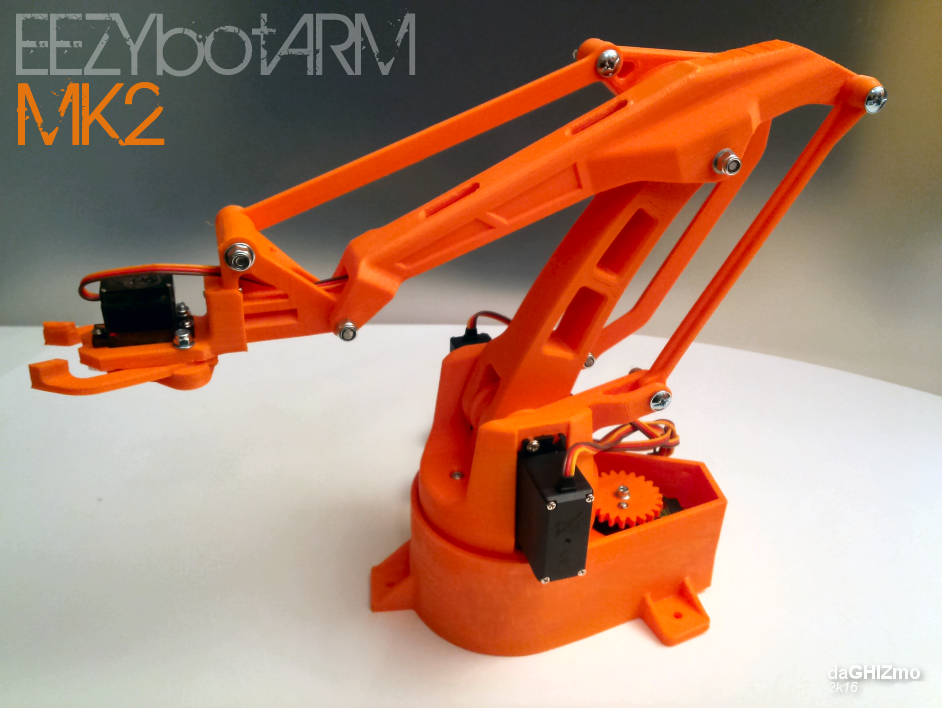
\includegraphics[width=0.8\linewidth]{image/rameno.png} 
			
		\end{figure}
		
		\vspace{0.02 \textheight}
		\begin{table}[h!]
			\begin{tabular}{ll}
				\textbf{Autor:} & \jmenoAutora\\ 
				\textbf{Obor:} & \kodOboru { } \obor\\
				\textbf{} & \zamereni\\
				\textbf{Třída:} & \trida\\
				\textbf{Školní rok:} & \skolniRok\\
			\end{tabular}
			
		\end{table}		
	}
	
\cleardoublepage %% Zalomení dvojstránky
	
%% Stránka obsahující poděkování a prohlášení
%%%%%%%%%%%%%%%%%%%%%%%%%%%%%%%%%%%%%%%%%%%%%%%%%%%%%%%%

%% Poděkování - nepovinné
%%%%%%%%%%%%%%%%%%%%%%%%%%%%
	
	\noindent{\large{\bfseries{Poděkování}\\}}
	\noindent Chci poděkovat panu učiteli Godovskému za poskytnutí veškerého hardware a konzultace během celé práci.
	
	\vspace*{0.7\textheight} %% Vertikální mezeru je možné upravit

%% Prohlášení - povinné
%%%%%%%%%%%%%%%%%%%%%%%%%%%%
	\noindent{\large{\bfseries{Prohlášení}\\}}  %% uprav si koncovky podle toho na jaký rod se cítíš, vypadá to pak lépe :) 
	\noindent{Prohlašuji, že jsem závěrečnou práci vypracovala samostatně a uvedla veškeré použité 
		informační zdroje.\\}
	\noindent{Souhlasím, aby tato studijní práce byla použita k výukovým a prezentačním účelům na Střední průmyslové a umělecké škole v Opavě, Praskova 399/8.}
	\vfill
	\noindent{V Opavě \datumOdevzdani\\}
	\noindent
	\begin{minipage}{\linewidth}
		\hspace{9.5cm} 
		\begin{tabular}{@{}p{6cm}@{}}
			\dotfill \\
			Podpis autora
		\end{tabular}
	\end{minipage}
	
	\cleardoublepage %% Zalomení dvojstránky

%% Stránka obsahující abstrakt (anotaci)
%%%%%%%%%%%%%%%%%%%%%%%%%%%%%%%%%%%%%%%%%%%%%%%%%%%%%%%%	

%% Abstrakt v češtině
%%%%%%%%%%%%%%%%%%%%%%%%%%%%
	\noindent{\Large{\bfseries{Abstrakt }\\}}
	\noindent 
	Výsledkem projektu je funkční pohyblivé rameno, které zvládá chytnout kuličku z~konce stavebnice a posune ji na začátek a také za dobře odvedenou práci se uklonit. Ovládané je gesty které jsou snímány kamerou notebooku. Hlavním aspektem projektu je kontrola jednotlivých servomotoru ramene pomocí gest. Kód který umožní zobrazovat  gesta je psaný v Pythonu, a holá pohyblivost ramene je obstarána Arduinem které využívá C++. 
	
	
	\vspace{18pt}
	
	\noindent{\large{\bfseries{Klíčová slova}}}
	
	\noindent poghyblivé rameno, gesta, Python, C++, Serva, Servomotory, knihovny, ukázky. 
	
	\vspace{18pt}

%% Abstrakt v angličtině
%%%%%%%%%%%%%%%%%%%%%%%%%%%%	
	\noindent{\Large{\bfseries{Abstract}}}
	
	\noindent The result of the project is a functional moving arm that manages to grab the ball from the end of the kit and move it to the beginning, as well as take a bow for a job well done. It is controlled by gestures that are captured by the laptop's camera. The main aspect of the project is the control of the individual servomotors of the arm using gestures. The code that allows the gestures to be displayed is written in Python, and the bare arm's mobility is handled by an Arduino which uses C++. 
	
	 %% přepiš!!
	
	\vspace{18pt}
	
	\noindent{\large{\bfseries{Keywords}}}
	
	\noindent moving arm, gestures, Python, C++, Servos, Servomotors, libraries, demos.
	
	\cleardoublepage %% Zalomení stránky

%% Stránka s generovaným obsahem
%%%%%%%%%%%%%%%%%%%%%%%%%%%%%%%%%%%%%%%	
	
	\tableofcontents %% Vygeneruje tabulku s obsahem

	\pagenumbering{arabic} %% Nastavení způsobu číslování stránek (alternativy roman | Roman)
	\setcounter{page}{1} %% Nastavení počitadla stránek

%% Stránka s úvodem - povinná část
%%%%%%%%%%%%%%%%%%%%%%%%%%%%%%%%%%%%%%%		
	\chapter*{Úvod}

	\addcontentsline{toc}{chapter}{Úvod}
	


Tato dokumentace detailně popisuje celkovou funkcionalitu mého projektu. Když jsme byli seznámeni s požadavky na ukončení čtvrtého ročníku ročníkovým projektem, rozhodla jsem se zaměřit svůj projekt především na oblast hardwaru. Po dlouhém a náročném průzkumu a s pomocí pana Godovského jsem nakonec zvolila robotické rameno pro svůj projekt. Bohužel, proces ovládání mě přivedl zejména k softwarovým aspektům.

Rameno je ovládáno pomocí předdefinovaných gest zachycených kamerou notebooku. Původně byl také zvažován koncept úplného ovládání ramene tak, aby kopírovalo pohyb lidské ruky. Nicméně k realizaci tohoto nápadu by bylo nutné dokoupit Pohyblivý senzor Kinect pro Xbox, což by bylo spojeno s významnými finančními náklady. Z tohoto důvodu jsem se rozhodla od tohoto přístupu ustoupit.

Cílem projektu bylo zprovoznit pohyb ramene celkem jednoduchým ale také efektivním způsobem. Díky tomu jsem si skvěle procvičila Python a C++. Motivoval mě ten pocit že to rameno rozpohybuji. 


V první kapitole naleznete seznam všech potřebných součástek pro sestavení samotného ramene. Samotnou fyzickou montáž jsem však neprováděla, a proto se budu věnovat zejména softwarovým aspektům. Tato část je doplněna krátkou teorií o využitých technologiích. V závěru kapitoly jsou uvedeny odkazy na všechny použité zdroje.
%Tipy k psaní úvodu
%Je povinný, nadpis neměňte, rozsah - max. 1 strana. 
%Tato část práce obsahuje: 
%* náhled do řešené problematiky, zdůvodnění volby problematiky, 
%* předem definované cíle práce, 
%* motivaci pro další čtení textu včetně stručného uvedení obsahu následujících kapitol 


\chapter{Princip fungování projektu}

Zde je strukturovaný náčrt fungování celého projektu. Kamera zachytává specifické gesto, a pomocí kódu využívajícího knihoven převádí obraz na nezbytné hodnoty, které jsou následně rozpoznány robotickým ramenem. Tyto hodnoty jsou poté předány do Arduina, který následně přiřazuje odpovídající signály na určité piny, aby serva ramene byla schopna rozpoznat a vykonat požadovanou akci.
\begin{figure}[h]
	
	\centering
	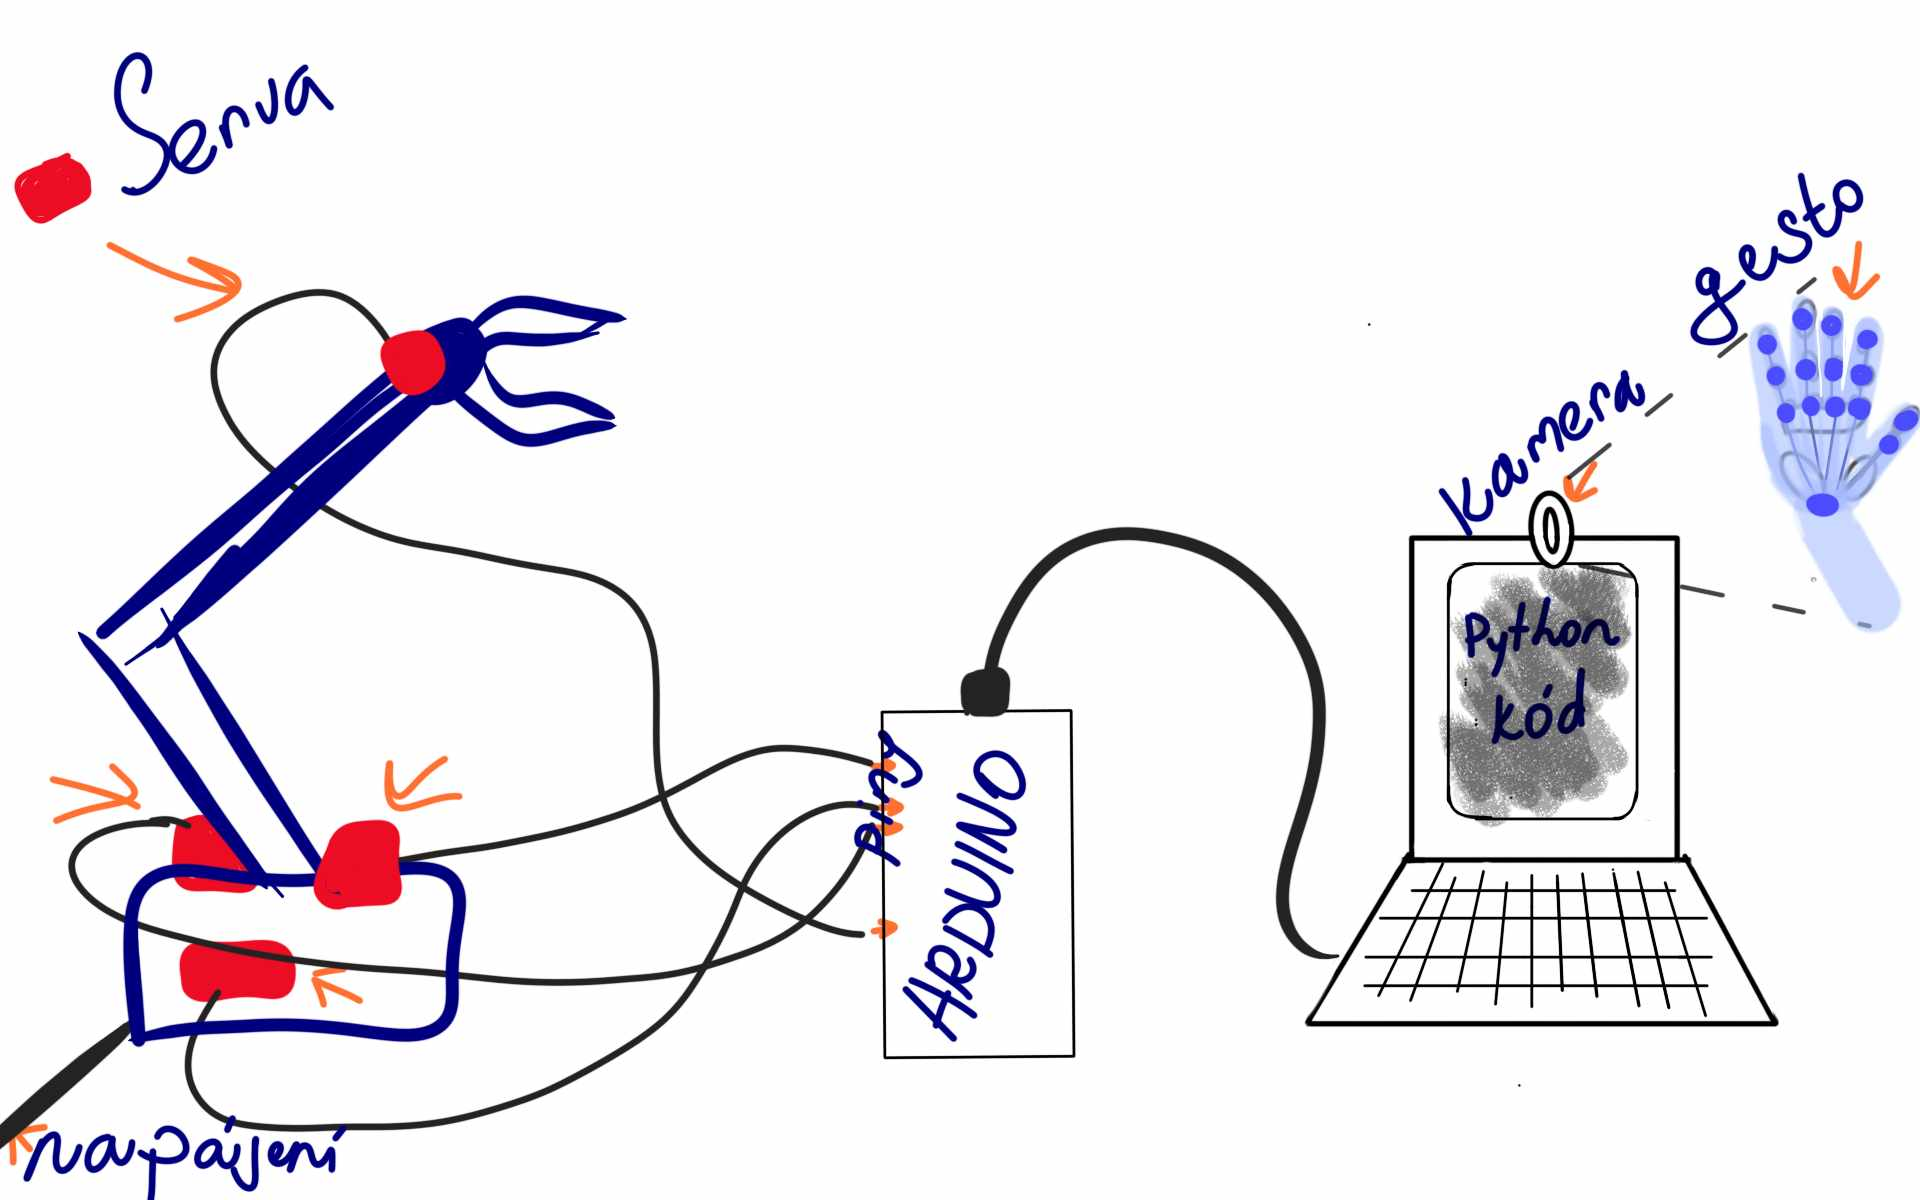
\includegraphics[width=0.9\linewidth]{image/princip.jpg} 
	
	
	\caption{Princip fungování projektu.} %% popisek obrázku, nezapomeň na citace!
	\label{fig:princip} %% označení až budeš chtít na obrázek odkazovat
\end{figure}


\chapter{Hardware}
	\section{Netištěné součástky}
Vzhledem k tomu, že jsem rameno nesestavovala, nemohu poskytnout detailní popis postupu montáže. Nicméně zde je výčet potřebných součástek:

\begin{itemize}
	\item	 3 - 955 nebo 946 servo
	\item 	1 - SG90 SERVO
	\item 	1 - Samojistná matice M6
	\item 	1 - Šroub M6x25
	\item 	2 - Samojistné matice M3
	\item 	2 - Šrouby M3 x 20
	\item 	1 - Šroub M3 x 10 se šestihrannou hlavou
	\item 	9 - Samojistné matice M4
	\item 	1 - Šroub M4 x 40
	\item 	1 - Šroub M4 x 30
	\item 	5 - Šroub M4 x 20
	\item 	1 - Závitová tyč M4 x 60mm
	\item 	1 - Závitová tyč M4 x 32 mm
	\item 	25 - Kulové koule o průměru 6 mm
	\item 	Ložisko 1 - 606zz
	\item 	Některé podložky M4
\end{itemize}


Návod na samotné sestavení ramene naleznete na \href{https://www.instructables.com/EEZYbotARM-Mk2-3D-Printed-Robot/}{tomhle odkazu} 
\newpage 


\subsection{Arduino nano 328}
\subsubsection{popis}

Arduino hraje klíčovou roli při oživení samotného hardwaru. Napsaný kód, který podrobněji popíšu v následující kapitole, je nahrán do mikrokontroléru pomocí USB kabelu. Díky správnému zapojení ramene se dosahuje bezproblémového fungování celého systému.


	\begin{figure}[h]
	
	\centering
	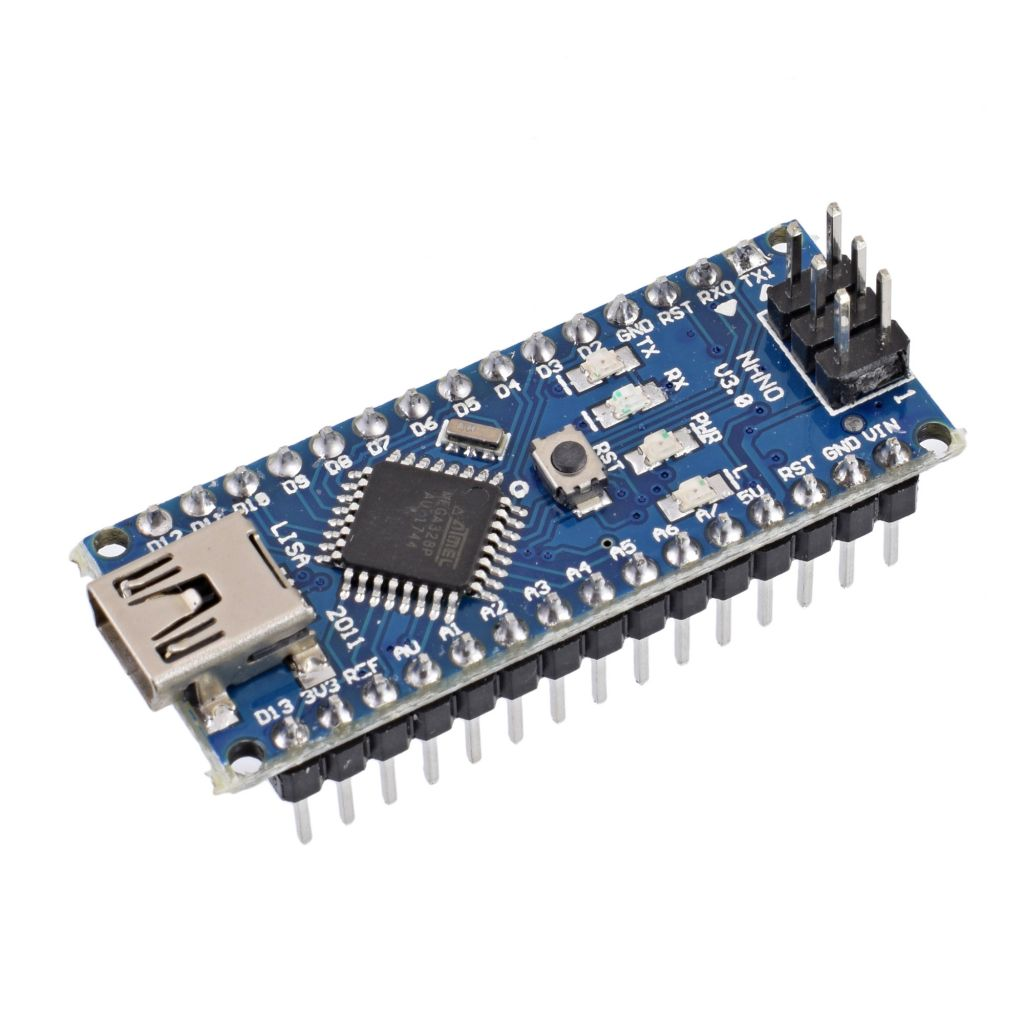
\includegraphics[width=0.6\linewidth]{image/arduino.jpg} 
	
	\caption{Arduino nano 328 } %% popisek obrázku, nezapomeň na citace!
	\label{fig:Arduino} %% označení až budeš chtít na obrázek odkazovat
\end{figure}

\newpage 

\subsection{Servomotory }
\subsubsection{Popis}
	
	Toto rameno zahrnuje tři velká serva a jedno menší. Každé servomotor disponuje třemi výstupy: kabelem určeným pro specifický port, záporným a kladným pólem. 
	\\ Nejmenší servomotor je umístěno v kleštičkách.
\begin{figure}[h]
	
	\centering
	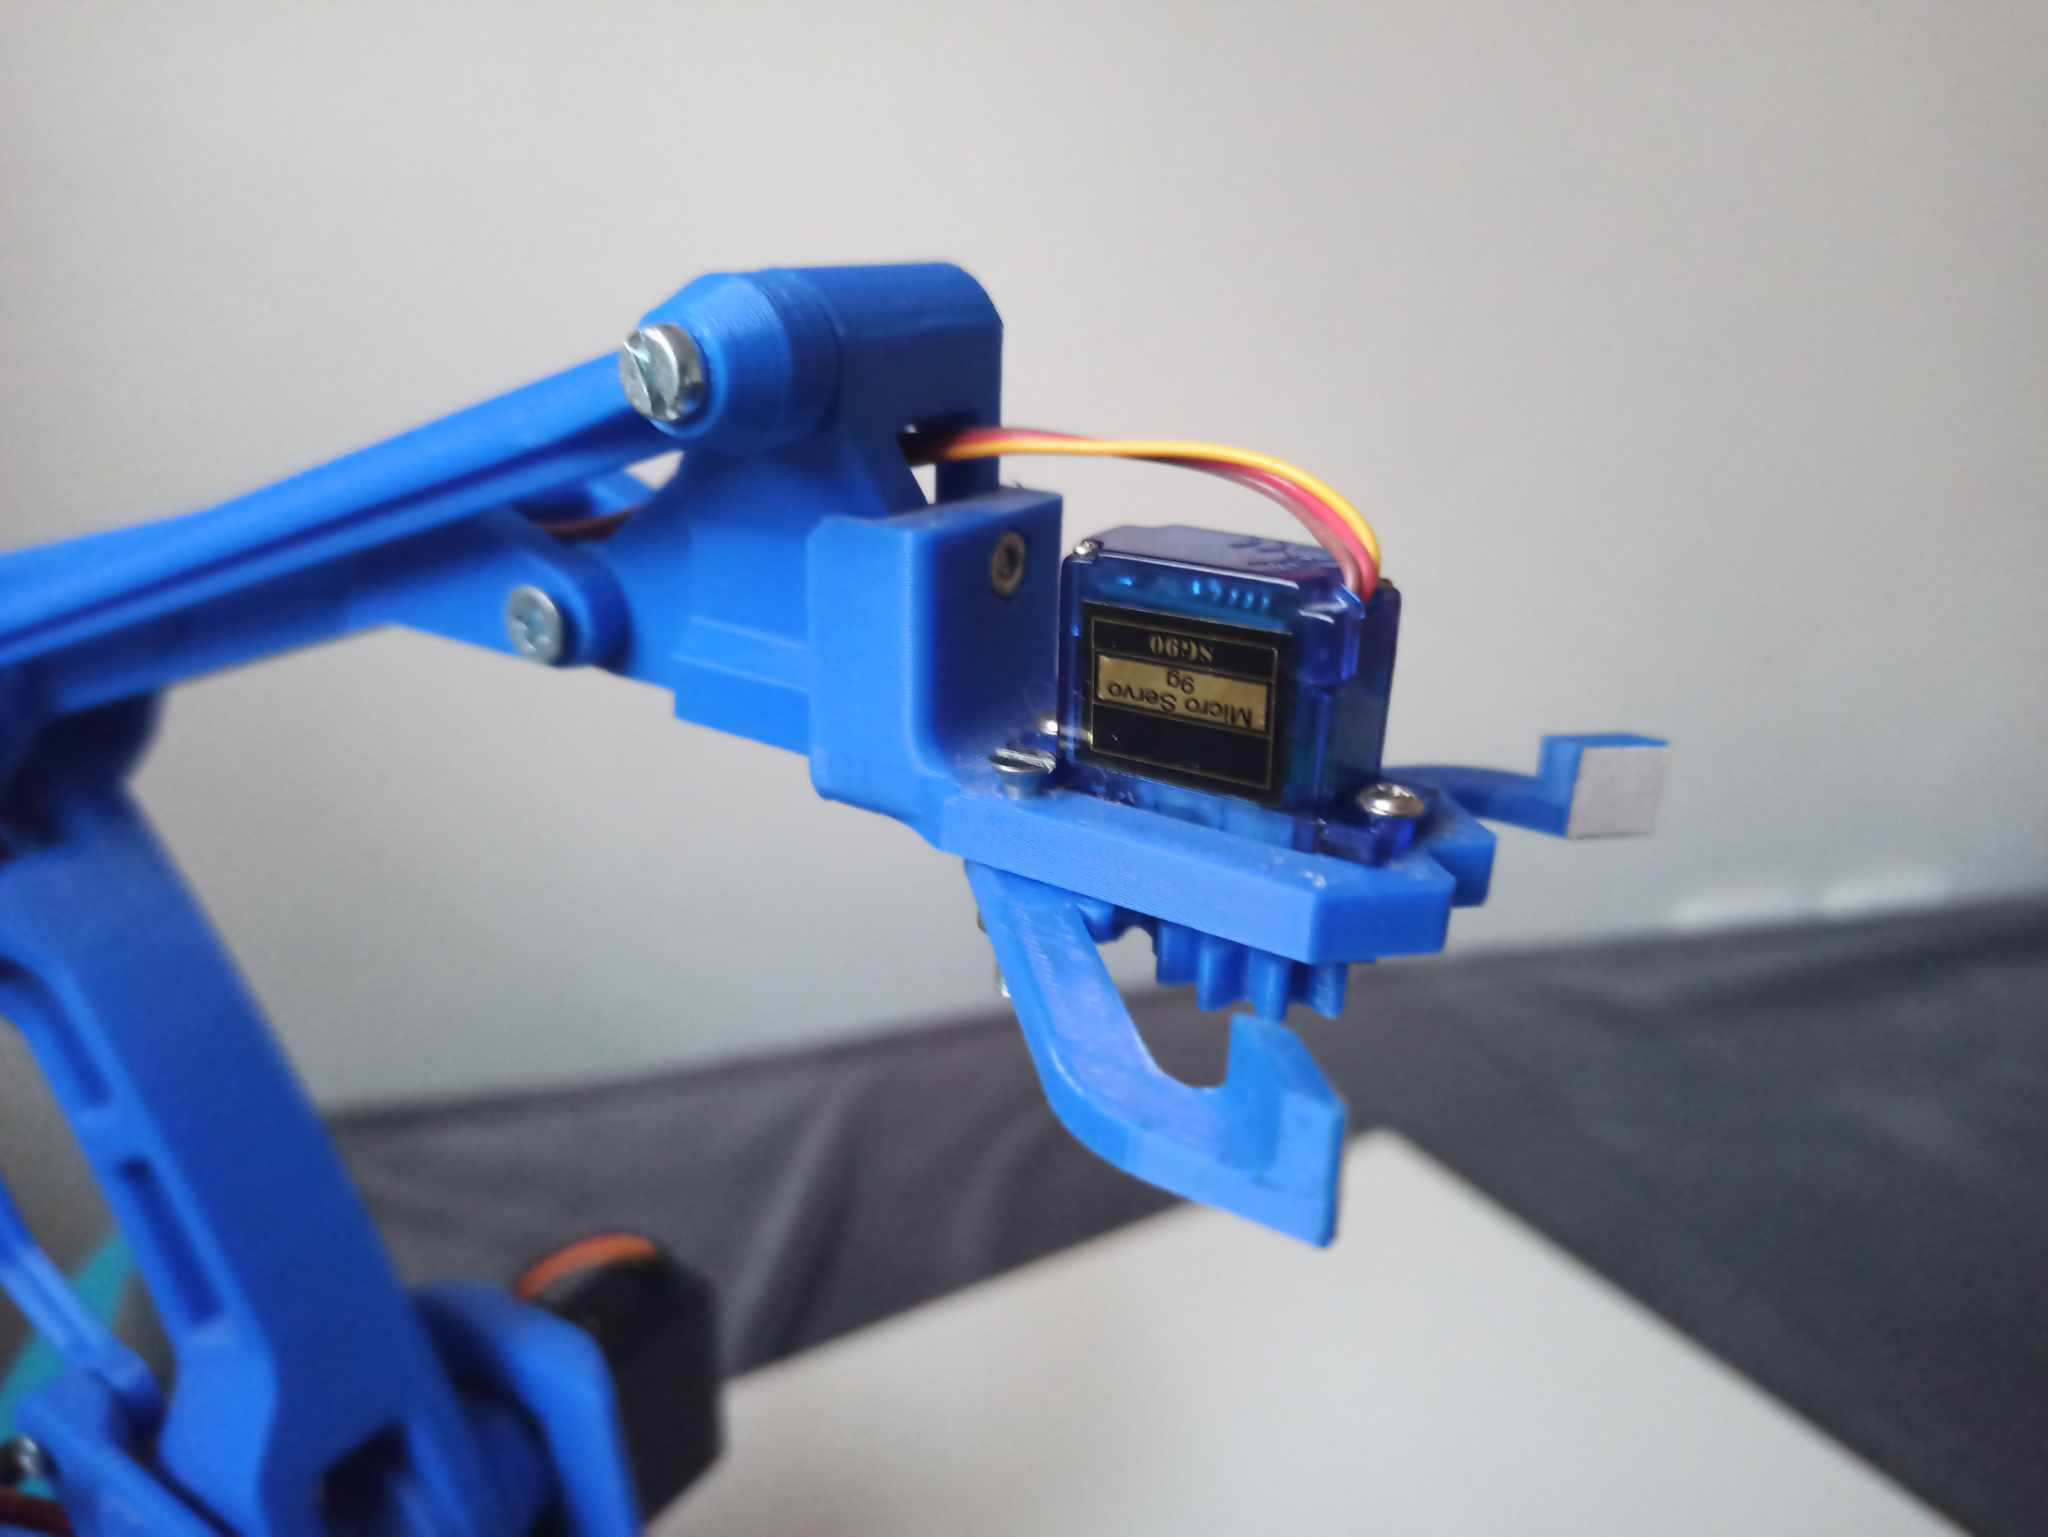
\includegraphics[width=0.5\linewidth]{image/kleste.jpg} 
	
	\caption{Servo nacházejíci se v kleštich ramene\cite{servo-kleste}.} %% popisek obrázku, nezapomeň na citace!
	\label{fig:Servo-kleste} %% označení až budeš chtít na obrázek odkazovat
\end{figure}

	Zbylé tři se zabývají rotací a pohyby nahoru-dolů, dopředu-dozadu

\begin{figure}[h]
	
	\centering
	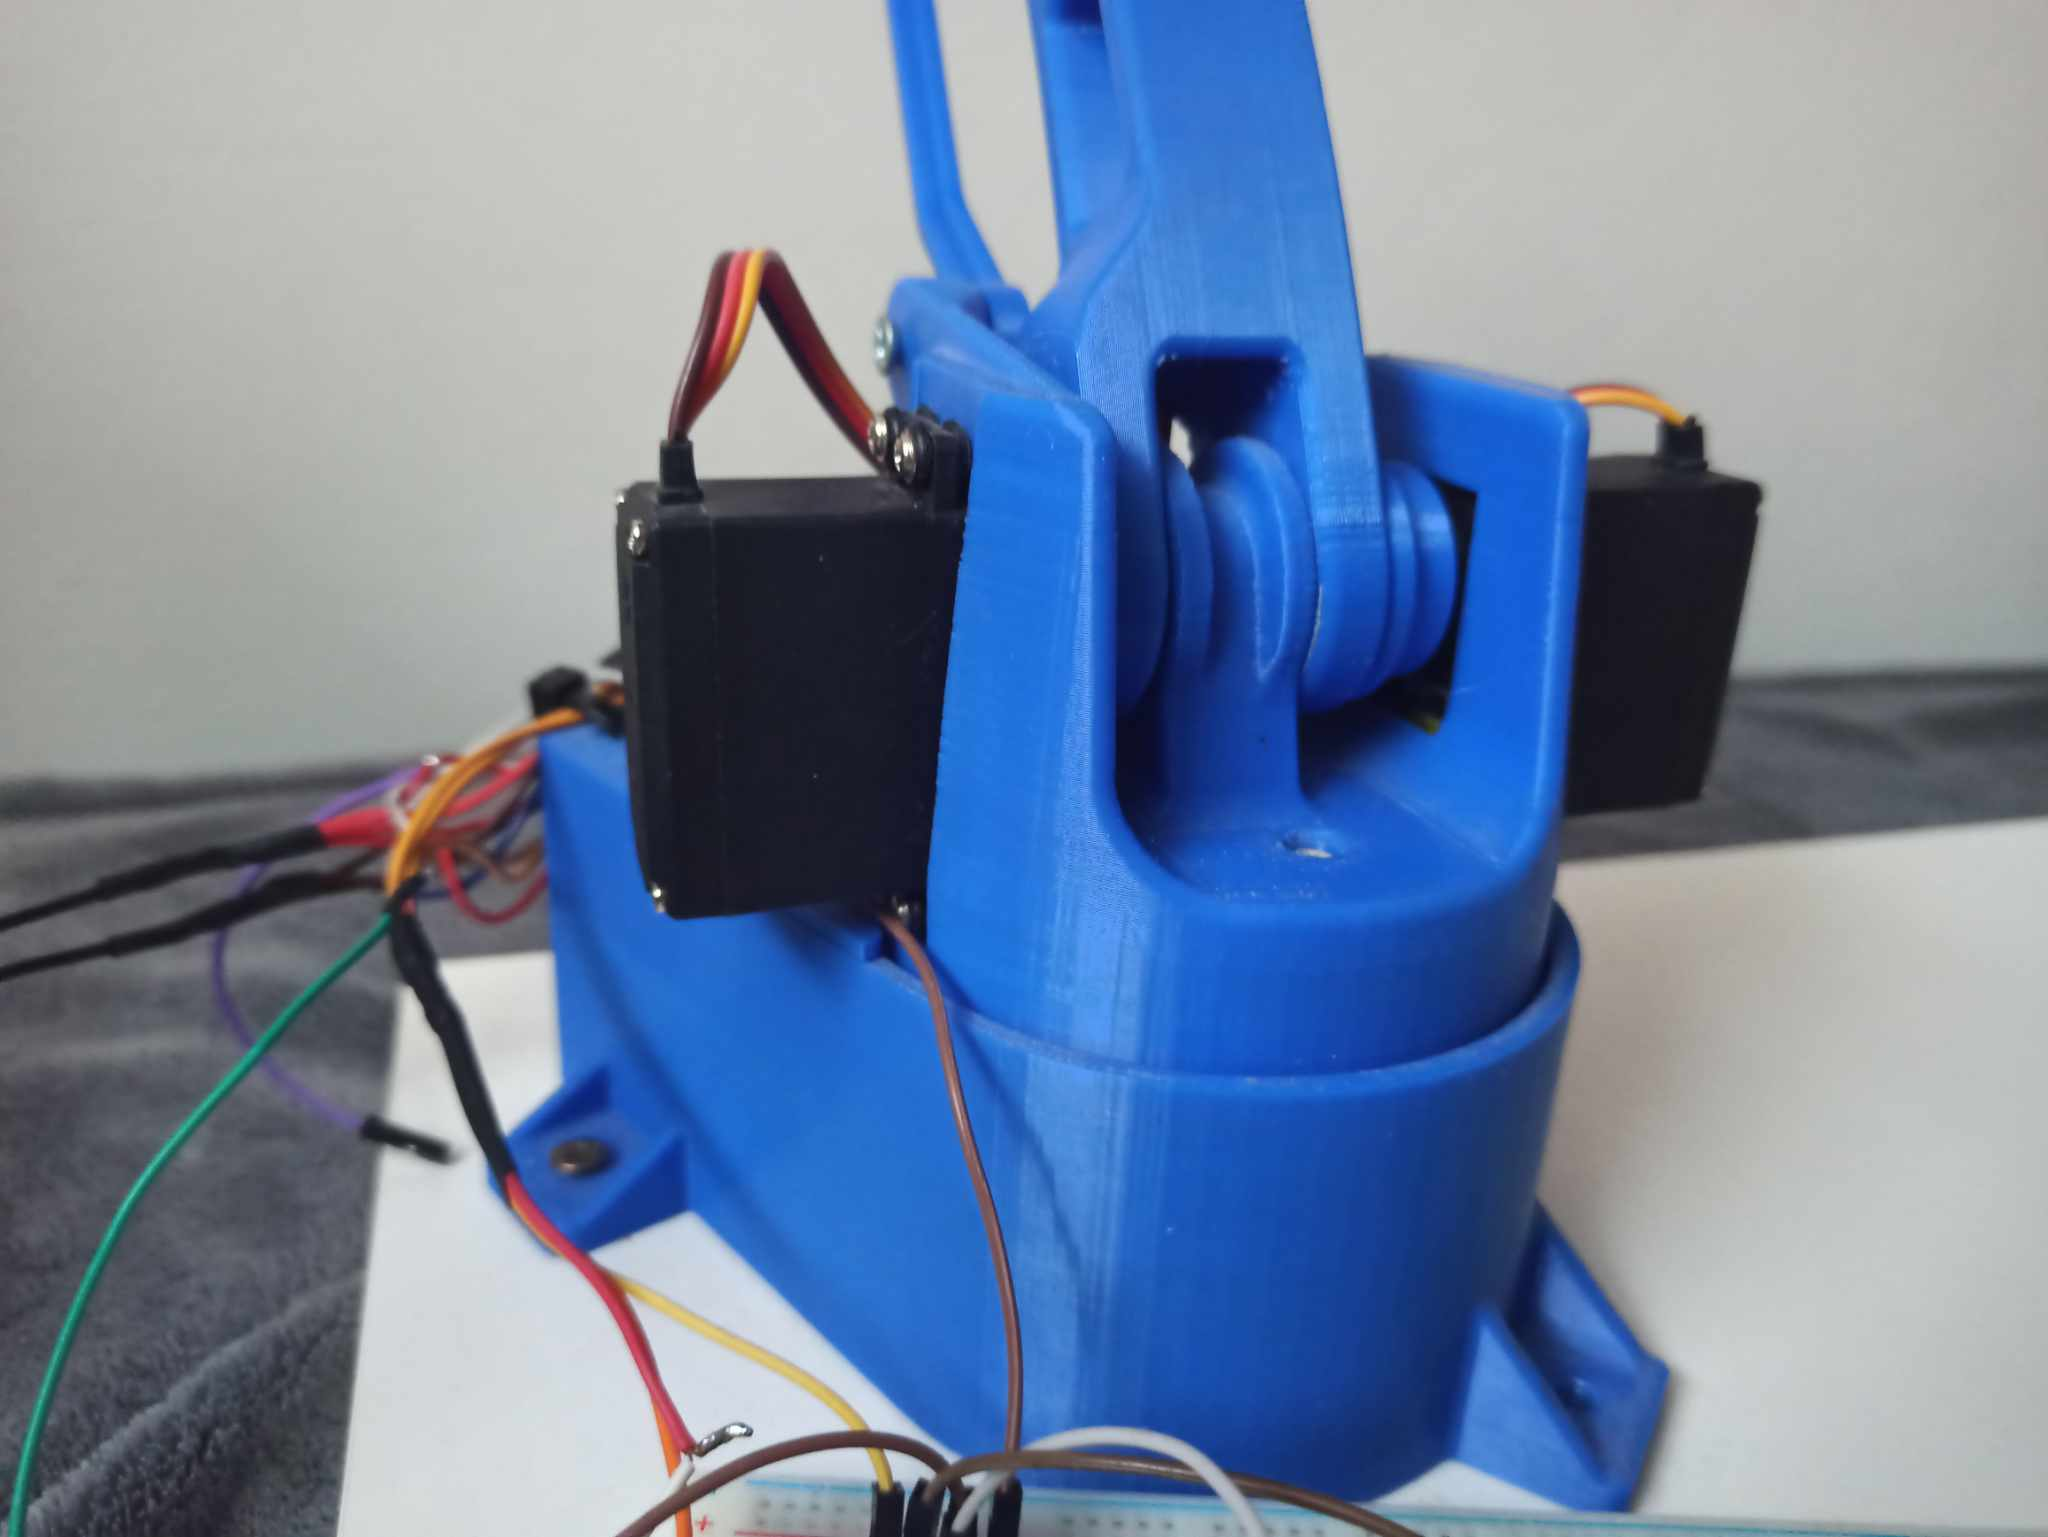
\includegraphics[width=0.5\linewidth]{image/serva.jpg} 
	
	\caption{Serva v těle ramene.} %% popisek obrázku, nezapomeň na citace!
	\label{fig:Serva} %% označení až budeš chtít na obrázek odkazovat
\end{figure}

\newpage

\subsection{Obvod}

\begin{figure}[h]
	
	\centering
	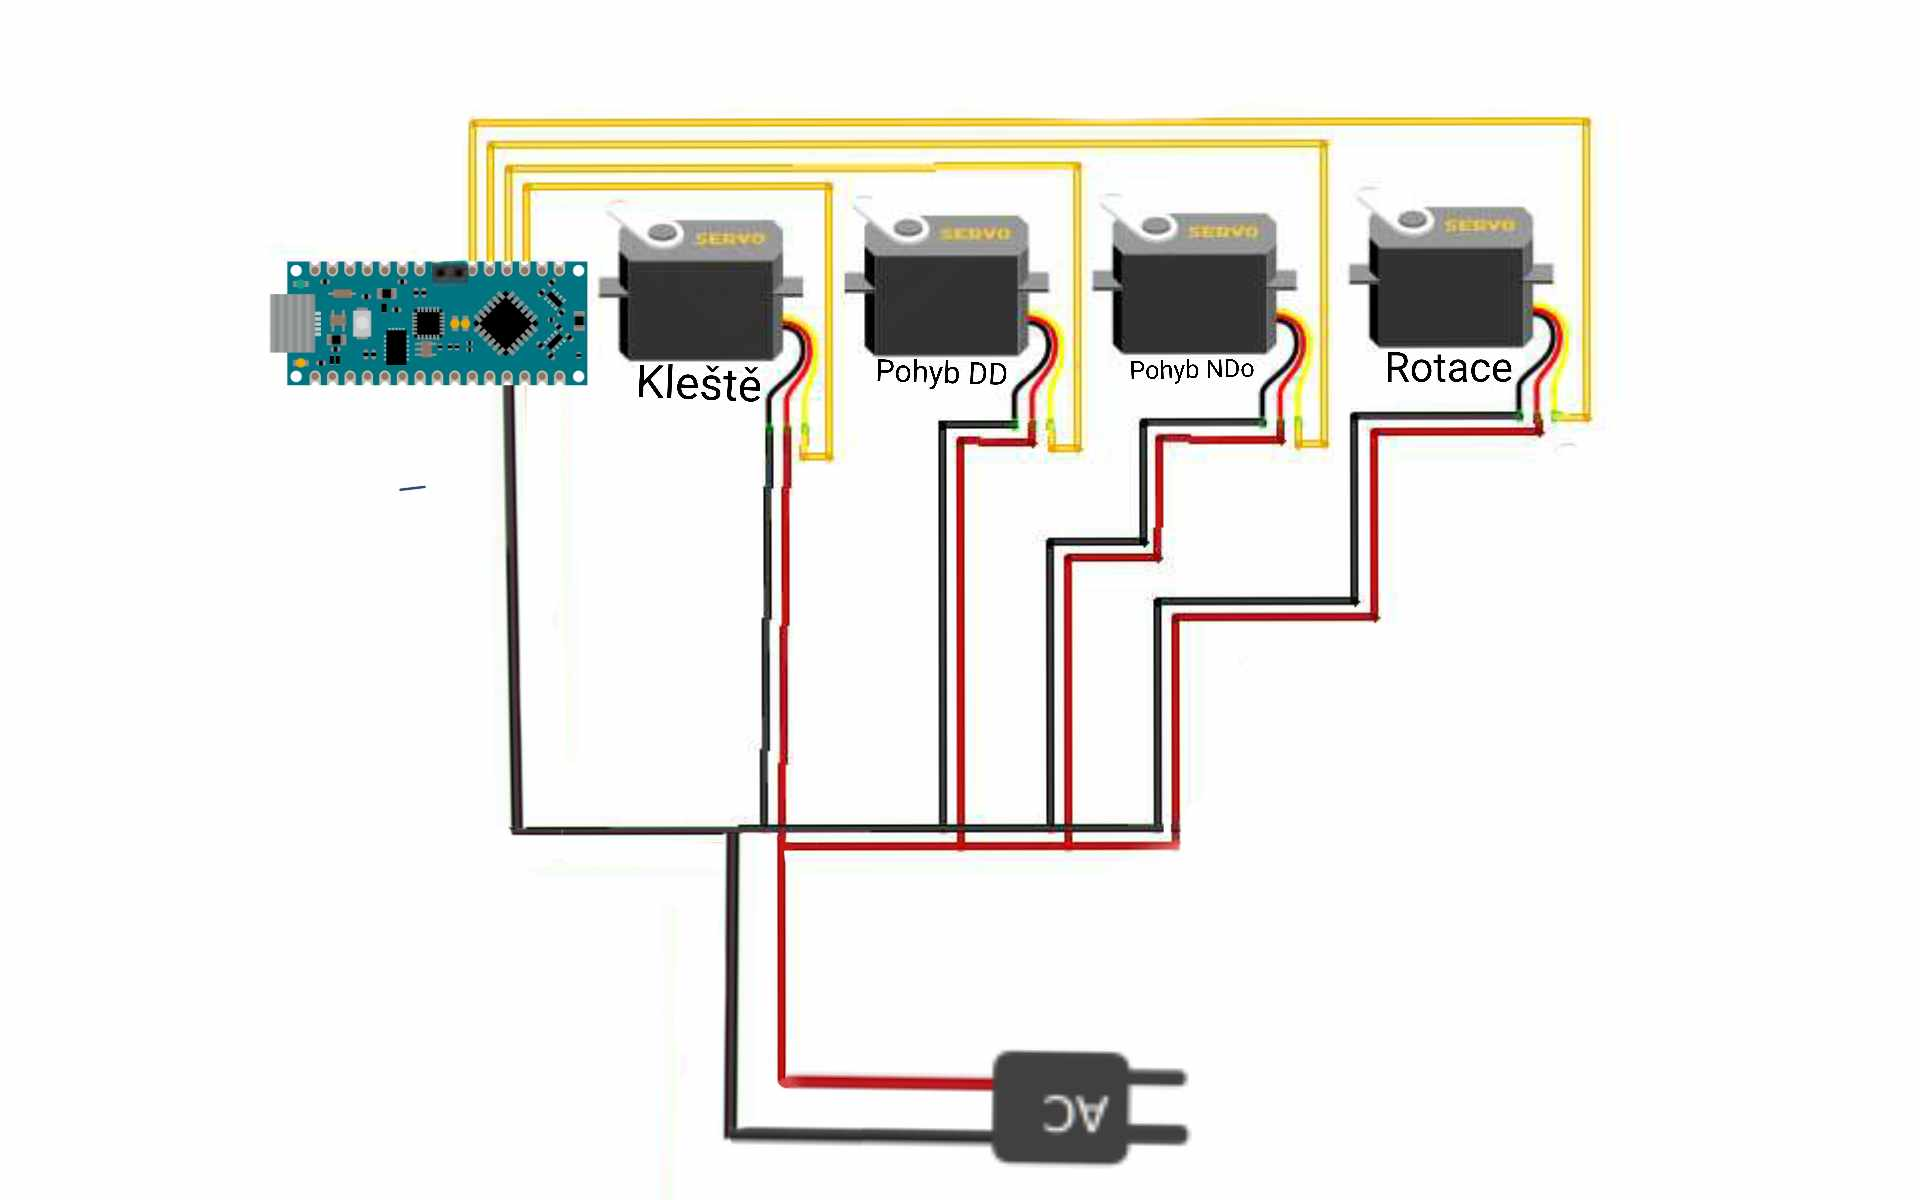
\includegraphics[width=0.9\linewidth]{image/obvod.jpg} 
	
	
	\caption{Zapojení ramene.} %% popisek obrázku, nezapomeň na citace!
	\label{fig:obvod} %% označení až budeš chtít na obrázek odkazovat
\end{figure}
\chapter{Software}

\section{Získání gest}
Začneme importem knihoven, a to \textbf{OpenCV}  \textbf{math} a \textbf{MediaPipe 0.10.8}  

\subsubsection{Knihovna OpenCV}

OpenCV představuje multiplatformní svobodnou knihovnu určenou pro manipulaci s obrazem. Tato knihovna je významnou měrou implementována v programovacím jazyce C++, nicméně je dodávána s Python obalem, což umožňuje její použití i v prostředí Pythonu. OpenCV nalézá uplatnění při zpracování obrazu z kamer a provádění úloh, jako je rozpoznávání psaného textu či obličejů.

Osobně jsem tuto knihovnu využila pro celkové zpracování obrazu z integrované kamery mého notebooku.

\begin{lstlisting}[style=Python, caption={Obraz, a jeho převedení do správného formátu}]
cap = cv2.VideoCapture(0)
...
image = cap.read()
imageRGB = cv2.cvtColor(image, cv2.COLOR_BGR2RGB)
results = hands.process(imageRGB)
\end{lstlisting}

Převede snímaný obraz do formátu RGB, který potřebujeme pro vykreslení pixelů ve správném pořadí.

\subsubsection{Knihovna MediaPipe}
Tato knihovna je specializována na detekci lidských částí těla, přičemž jsem se v rámci svého projektu zaměřila výhradně na detekci dlaní. Pro účely této detekce vyžaduje knihovna orientační body ruky. Model orientačních bodů pro ruku je schopen předpovídat 21 přesných souřadnic pro umístění každého orientačního bodu na ruce.



\begin{figure}[h]
	
	\centering
	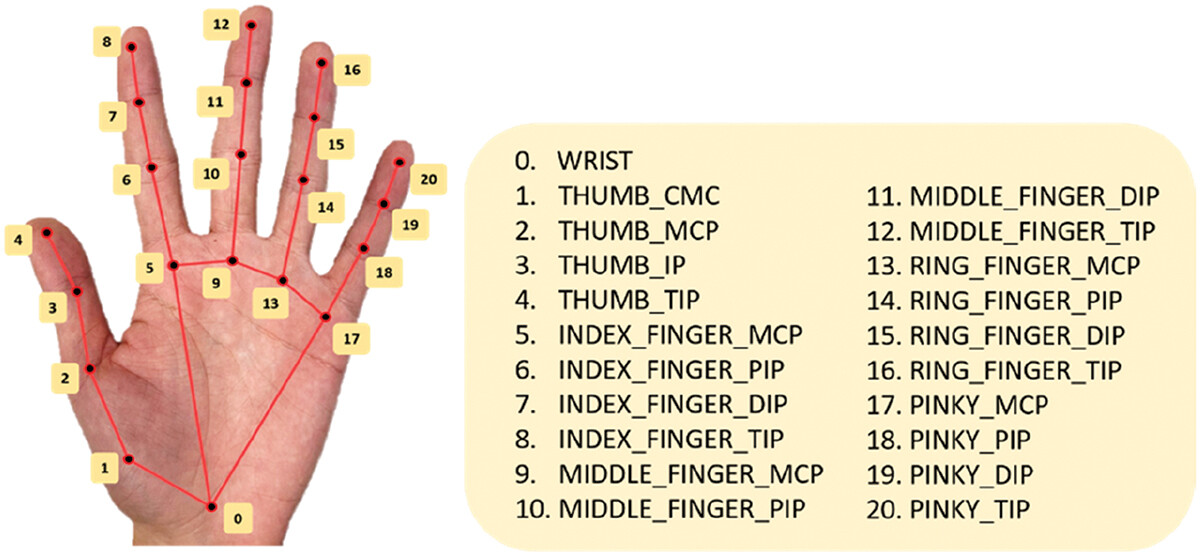
\includegraphics[width=0.8\linewidth]{image/orientacniBody.jpg} 
	
	
	\caption{Orientacni body dlaně.} %% popisek obrázku, nezapomeň na citace!
	\label{fig:obvod} %% označení až budeš chtít na obrázek odkazovat
\end{figure}

\subsubsection{Knihovna math}

Ve spolupráci s výše zmíněnou knihovnou jsem získala souřadnice jednotlivých kloubů, což umožnilo přesné zachycení postavení ruky. Kromě toho jsem prováděla další výpočty pro určení vzdálenosti mezi prsty, což bylo nezbytné pro správné identifikování gesta potřebného k ovládání kleštiček.

\begin{figure}[h]
	
	\centering
	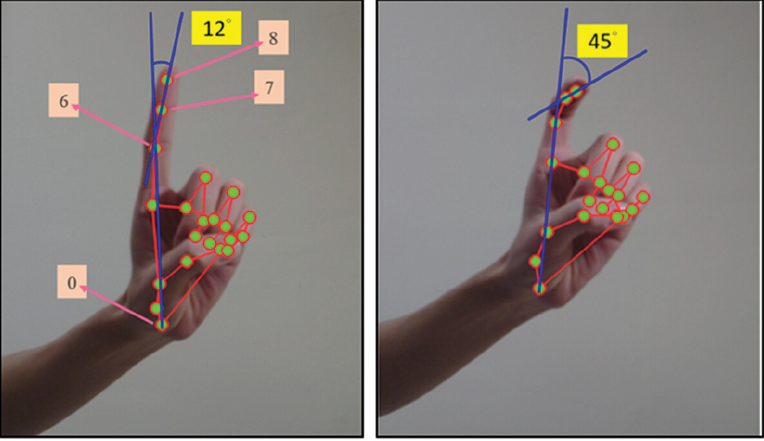
\includegraphics[width=0.4\linewidth]{image/prikladGesta.PNG} 
	
	
	\caption{Použití úhlu v gestech.} %% popisek obrázku, nezapomeň na citace!
	\label{fig:uhlyVGestech} %% označení až budeš chtít na obrázek odkazovat
\end{figure}
\begin{figure}[h]
	
	\centering
	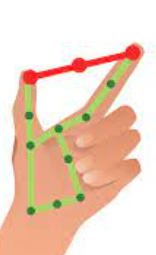
\includegraphics[width=0.2\linewidth]{image/vzdalenost.PNG} 
	
	
	\caption{Použití měření vzdálenosti v gestech.} %% popisek obrázku, nezapomeň na citace!
	\label{fig:vzdalenost} %% označení až budeš chtít na obrázek odkazovat
\end{figure}



\newpage

\section{Ověření funkčnostní ramene}
Předtím, než jsem mohla začít s implementací nápadu na pohyblivé rameno, bylo nezbytné ověřit jeho funkčnost a porozumět pohybu jednotlivých částí. K tomuto účelu jsem využila jednoduchý kód. Postupně jsem připojovala jednotlivé drátky k desce s Arduino a zjišťovala, který drát odpovídá za kterou část a jak se tato část pohybuje. Narazila jsem na jednu komplikaci, kdy servomotory stávkovaly, když jsem posílala extrémní hodnoty (0, 180). Po upravení rozsahu v intervalu ve funkci se vše dostalo do pořádku.
\begin{lstlisting}[style=Python, caption={Ukázka kódu k ověření funkčnosti}]
#include <Servo.h>

Servo myservo;  

int pos = 0;    
void setup() {
	myservo.attach(9);  
}

void loop() {
	for (pos = 2; pos <= 160; pos += 1) { 
		myservo.write(pos);             
		delay(15);                      
	}
	for (pos = 160; pos >= 2; pos -= 1) {
		myservo.write(pos);            
		delay(15);                       
	}
}
\end{lstlisting}

\newpage

\section{Práce s Arduinem}
\subsection{Inicializace hodnot}
První věc, kterou musíme vzít v úvahu, je, že nezbytně potřebujeme mít na svém počítači program Python a také PySerial. Většinu kódu v Pythonu se dá sehnat na internetu a odkazy na ty stránky naleznete níže v použité literatuře. 
Takže se jdeme přesunout k popisu.
Pro kód v C++ je na začátek potřeba inicializovat veškeré potřebné hodnoty.
např:

\begin{lstlisting}[style=Python, caption={Inicializace potřebných hodnot}]
const int min= 2;  // minimalní hodnota rozmezí pro vzdálenost
const int max = 160; // maximalní hodnota rozmezí pro vvzdálenost

bool end;
int data = 0;
int serialData = 0;
bool changeMode;
int mode;
const int servoPose = 6; //kolik stavu má rameno
const int servoCount = 4; // počet serv

Servo servo[4]; // pole pro serva 
const byte servoPins [] = {2,3,4,5}; //piny pro serva
\end{lstlisting}


\begin{itemize}
	\item 
	Vzhledem k tomu, že pro řízení pohybu kleští potřebujeme hodnoty v rozmezí od 0 do 180, je nutné přemapovat posílanou vzdálenost. K tomu účelu využívám proměnné "min" a "max", které určují rozsah posílaných hodnot.
	\item Dále je tu proměnná "changeMode", která slouží k přepínání mezi režimem snímání počtu prstů a režimem měření vzdálenosti mezi prsty.
\begin{figure}[h]
	
	\centering
	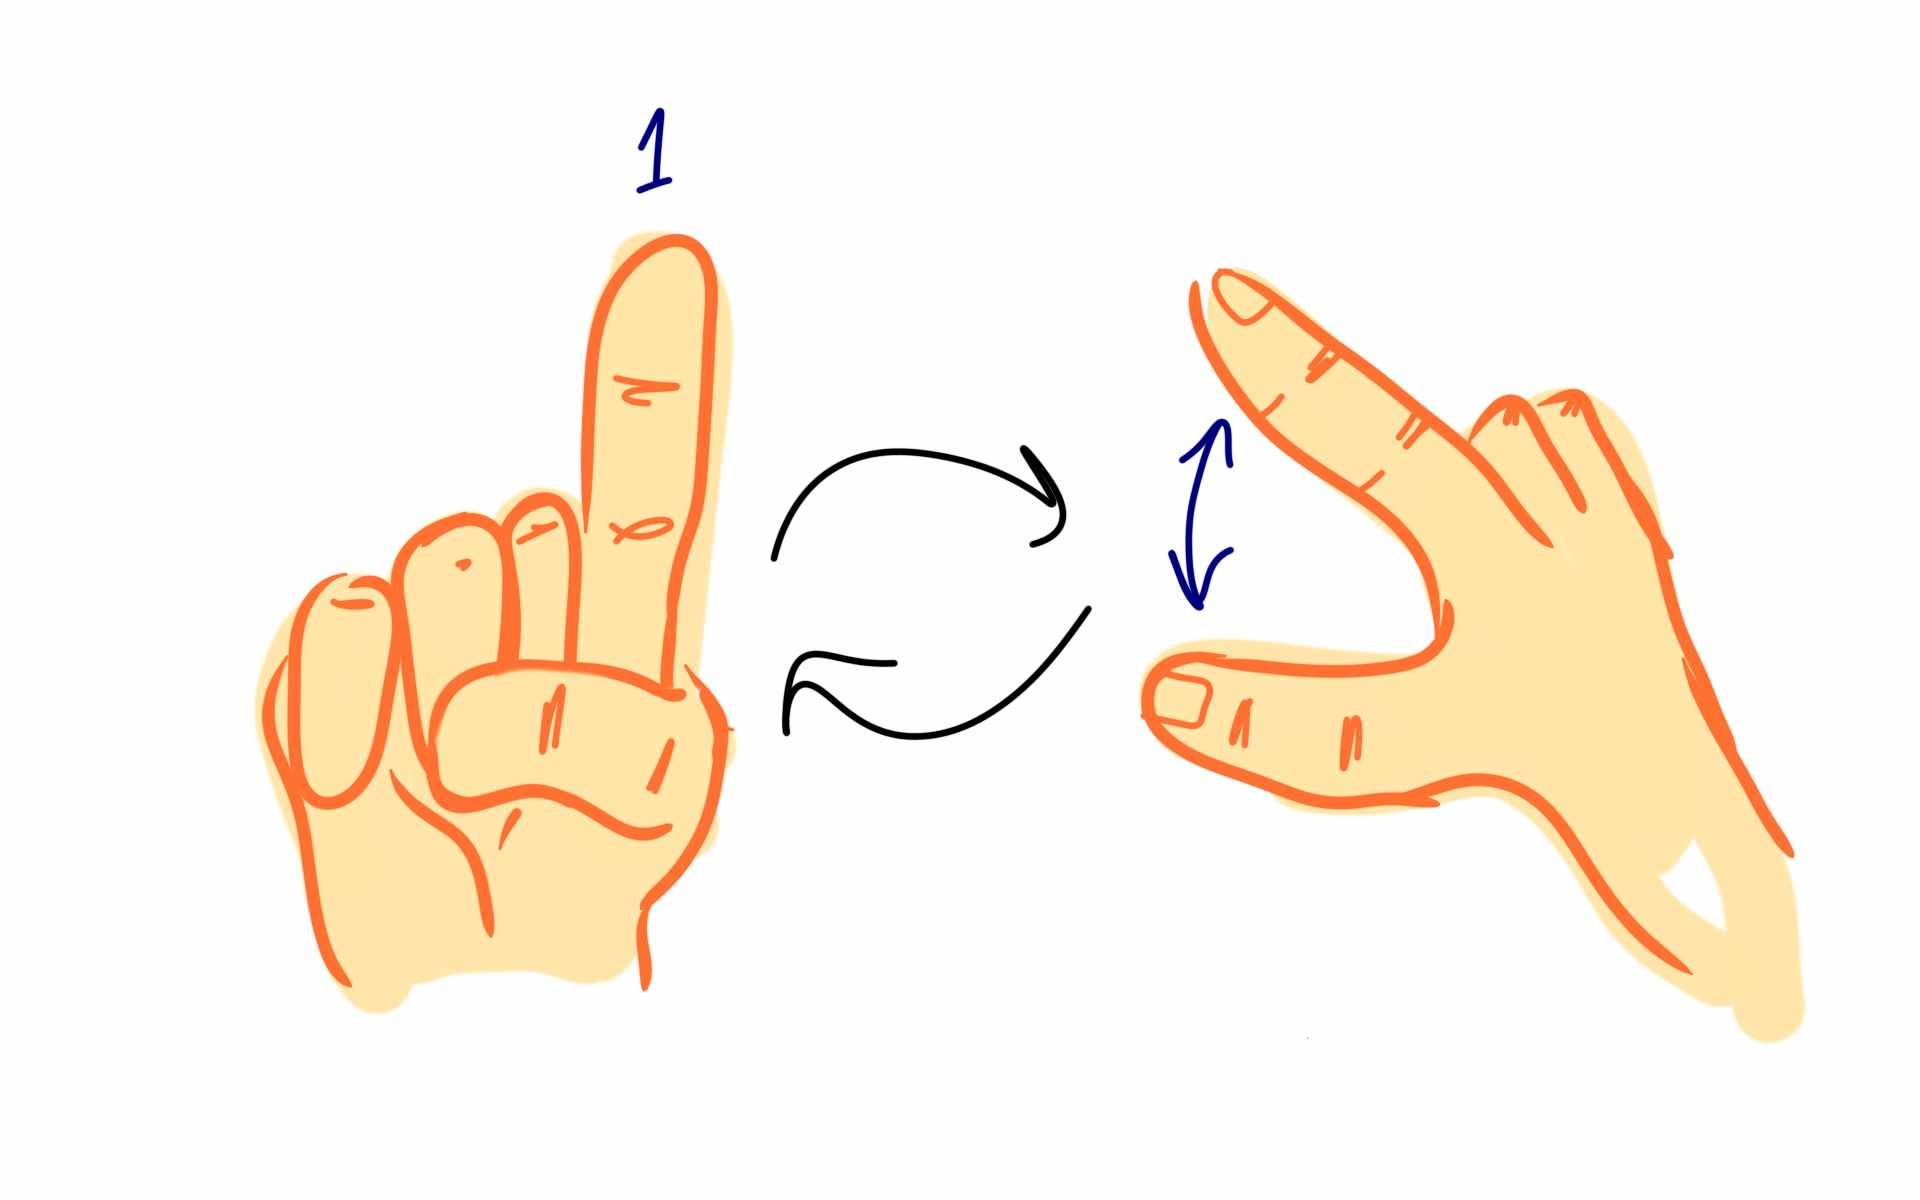
\includegraphics[width=0.3\linewidth]{image/mody.jpg} 
	
	
	\caption{Dvá módy pro kontrolu ramene.} %% popisek obrázku, nezapomeň na citace!
	\label{fig:uhlyVGestech} %% označení až budeš chtít na obrázek odkazovat
\end{figure}
\item   V proměnné "servoPos" je uložen počet všech možných stavů, ve kterých se může nacházet mé rameno.
\item Vzhledem k tomu, že má rameno 4 servomotory, vytvořila jsem pro ně pole. Každý servomotor vyžaduje svůj vlastní pin, který je následně specifikován v proměnné "servoPins".
	
\end{itemize}



\begin{lstlisting}[style=Python, caption={Podmínka pro přepínání módu}]
if(j == (servoMoves[data][0] - 1)) {
	if(data == 0 || data == 1) {
		changeMode = true;
		mode = data;
	}
\end{lstlisting}

\begin{itemize}
		\item Tato jednoduchá podmínka byla vytvořena pro kontrolu aktuální polohy ramene. Pokud se rameno nachází v horní nebo dolní poloze, dojde k přepnutí režimu pro měření vzdálenosti. To umožňuje manipulaci s ramenem, například pro chycení nebo pustení kuličky.

	
\end{itemize}
	
\begin{lstlisting}[style=Python, caption={Dvourozměrné pole na potřebné hodnoty}]
	 int servoValues [13] [3] = {
		{20,50,20},  //puvodni stav 
		{170,80,45}, //dole sběr kuličky cast1
		{123,113,45}, //dolu sběr kuličky cast2
		...
		{123,130,133},  //uklona cast2
	};
		\end{lstlisting}
		
\begin{itemize}
	\item Dále používáme dvourozměrné pole pro uložení hodnot pro servomotory. Hodnoty jsou vždy uspořádány ve třech sloupcích v jednom řádku, jelikož pro ovládání servomotorů v kleštích jsou potřebné odlišné hodnoty.
	
	
	
	

			
	\end{itemize}
	
\begin{lstlisting}[style=Python, caption={Další pole pro několik hodnot }]
	int servoMoves [servoPose] [3] = {
		{2,1,500}, //dolu ke kulice 1
		{2,3,500}, //nahoru ke kulice 2
		{5,5,700}, //ne  3
	...
	};	
	\end{lstlisting}
	
	\begin{itemize}
		\item Následující pole obsahuje několik různých hodnot. Na prvním místě je počet opakování pohybů, na druhém místě je pořadí hodnot pro servomotory z předchozího pole. Poslední hodnota v poli určuje časový odstup (delay).
		
		
		
		
		
		
		
		
	\end{itemize}

\begin{lstlisting}[style=Python, caption={Funkce na rozpohybocání ramene}]	
	void move(int data) {
		int cycle = 0;
		for(int j = 0 ; j < servoMoves[data][0];j++) {
			for(int i = 1; i < servoCount;i++) servo[i].write(servoValues[
											(servoMoves[data][1])+cycle][i - 1]);
			cycle++;
			if(cycle > 1) cycle=0;
			if(j == (servoMoves[data][0] - 1)) {
				if(data == 0 || data == 1) {
					changeMode = true;
					mode = data;
				}
				end = true;
				Serial.begin(9600);
			}
			delay(servoMoves[data][2]);
		}
	}
	
	\end{lstlisting}
	
	\begin{itemize}
		\item Jedná se o jednu z klíčových funkcí, která slouží k pohybu ramena. Jakmile je načtena jedna hodnota, funkce postupuje v cyklu o jeden prvek dál v poli "servoValues", dokud nedojde na konec. Poté se zkontroluje, zda jsou data rovna 0 nebo 1, což signalizuje, zda se rameno nachází v pozici u kuličky. V případě potvrzení této pozice se změní hodnota proměnné "changeMode" a přepne se na režim měření vzdálenosti mezi prsty.
		
	\end{itemize}
	
\newpage
	
\subsection{Manuál na  ovládání}

\begin{figure}[h]
	
	\centering
	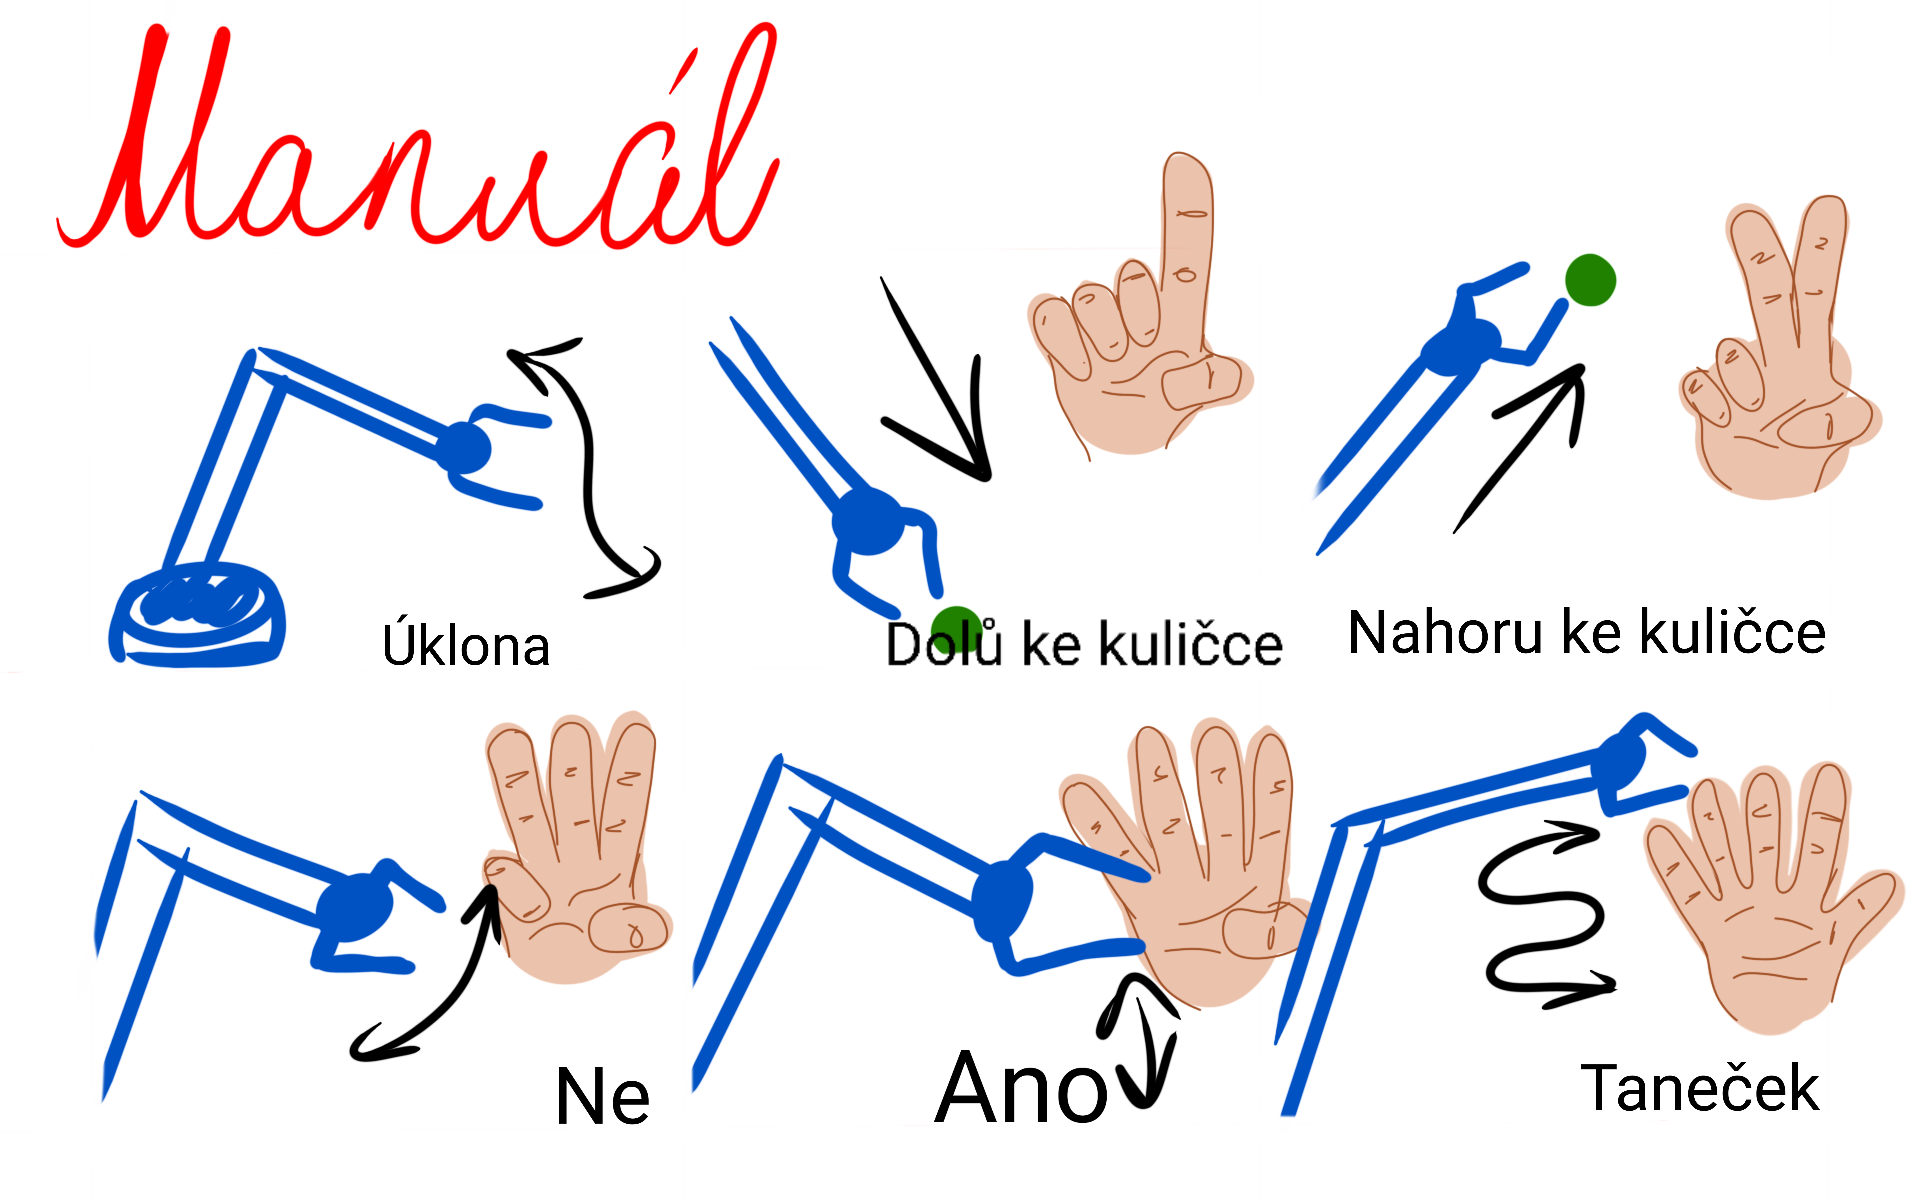
\includegraphics[width=0.8\linewidth]{image/manual.png} 
	
	
	\caption{Dvá módy pro kontrolu ramene.} %% popisek obrázku, nezapomeň na citace!
	\label{fig:uhlyVGestech} %% označení až budeš chtít na obrázek odkazovat
\end{figure}
	
	
	
	
	
	\chapter*{Závěr}
	\addcontentsline{toc}{chapter}{Závěr}
	
	Cílem celé práce bylo dosáhnout pohybu ramene a získat lepší porozumění fungování příslušných knihoven. Ve finální verzi je rameno schopno úspěšně uchopit kuličku a přesunout ji z konce na začátek. Celý projekt byl implementován pomocí kombinace jazyků Python a C++. Možné využití tohoto projektu může být rozmanité, například v továrnách, skladech, v nanochirurgii nebo jako vzdělávací hračka.
	
	Podařilo se mi dosáhnout původního cíle a rameno nyní pracuje tak, jak jsem si představovala na začátku vývoje. I přestože má můj kód určité nedostatky v optimalizaci, věřím, že by mohl být v budoucnu vylepšen. Rovněž plánuji detailněji studovat knihovnu OpenCV a prozkoumat další její funkce.
	
	
	
	
	
	
	
	
	odkaz na github: https://github.com/Sofjaklopcova/maturita
	
	%% literatura
	\renewcommand\bibname{Seznam použitých informačních zdrojů}
	\begin{thebibliography}{99}
		\addcontentsline{toc}{chapter}{Seznam použitých zrdojů}
		\bibitem{sablonaSOC}{Základní informace o gestech} [Online].  2023 CEMI MBA Studies s.r.o. [cit. 2020-08-24]. Dostupné z: \url{https://www.cemi.cz/blog/neverbalni-komunikace-co-prozradi-gesta}
		
		\bibitem{LaTeXprirucka} {Typy gest v běžném životě} [online]. 1998 [cit. 2020-08-24]. Dostupné z: \url{https://orangeacademy.cz/clanky/rec-tela/}
		
		\bibitem{wikibooksLaTeX} Řeč tela a znakový jazyk, 2023, Slůně - svět jazyků, s.r.o. Dostupné z: \url{https://www.slune.cz/aktualita/znakovy-jazyk/}
		
		\bibitem{wikibooksLaTeX} Knihovna math v pythonu Copyright © 2023 itnetwork.cz.
	 \url{https://www.itnetwork.cz/python/zaklady/python-tutorial-knihovny-math-a-random}
	 	\bibitem{wikibooksLaTeX} Knihovna opencv v pythonu Copyright © 2023 itnetwork.cz.
	 \url{https://www.python-programator.cz/clanky/python-pro-zpracovani-obrazu-opencv}
	 \bibitem{wikibooksLaTeX} Komunikace s arduinem  © 2023 Arduino
	 \url{https://projecthub.arduino.cc/ansh2919/serial-communication-between-python-and-arduino-663756}
	 \bibitem{wikibooksLaTeX}Komunikace s arduinem 2 Copyright © 2023 Circuit Digest. All rights reserved.
	 \url{https://circuitdigest.com/microcontroller-projects/arduino-python-tutorial}
	  \bibitem{© 2023 Arduino}Zkouška funkčnosti 
	 \url{https://docs.arduino.cc/learn/electronics/servo-motors}
	  \bibitem{wikibooksLaTeX}Zkouška funkčnosti 
	 \url{https://problemsolvingwithpython.com/11-Python-and-External-Hardware/11.03-Controlling-an-LED/}
	 
	 
	 
		
		
		
	
	\end{thebibliography}
	
	%% obrázky 
	\listoffigures
	

	
	\appendix %% začínají přílohy
	
	\titleformat{\chapter}[block]{\scshape\bfseries\LARGE}{Příloha \thechapter}{10pt}{\vspace{0pt}}[\vspace{-22pt}] %% nastavení nadpisu u příloh
	
	

	
	
\end{document}